% Graphic for TeX using PGF
% Title: C:\DEV\PHILLIPO.jl\documentation\Figuras\fluxograma_GiD.dia
% Creator: Dia v0.97.2
% CreationDate: Sun Jun 25 20:27:10 2023
% For: lucas
% \usepackage{tikz}
% The following commands are not supported in PSTricks at present
% We define them conditionally, so when they are implemented,
% this pgf file will use them.
\ifx\du\undefined
  \newlength{\du}
\fi
\setlength{\du}{15\unitlength}
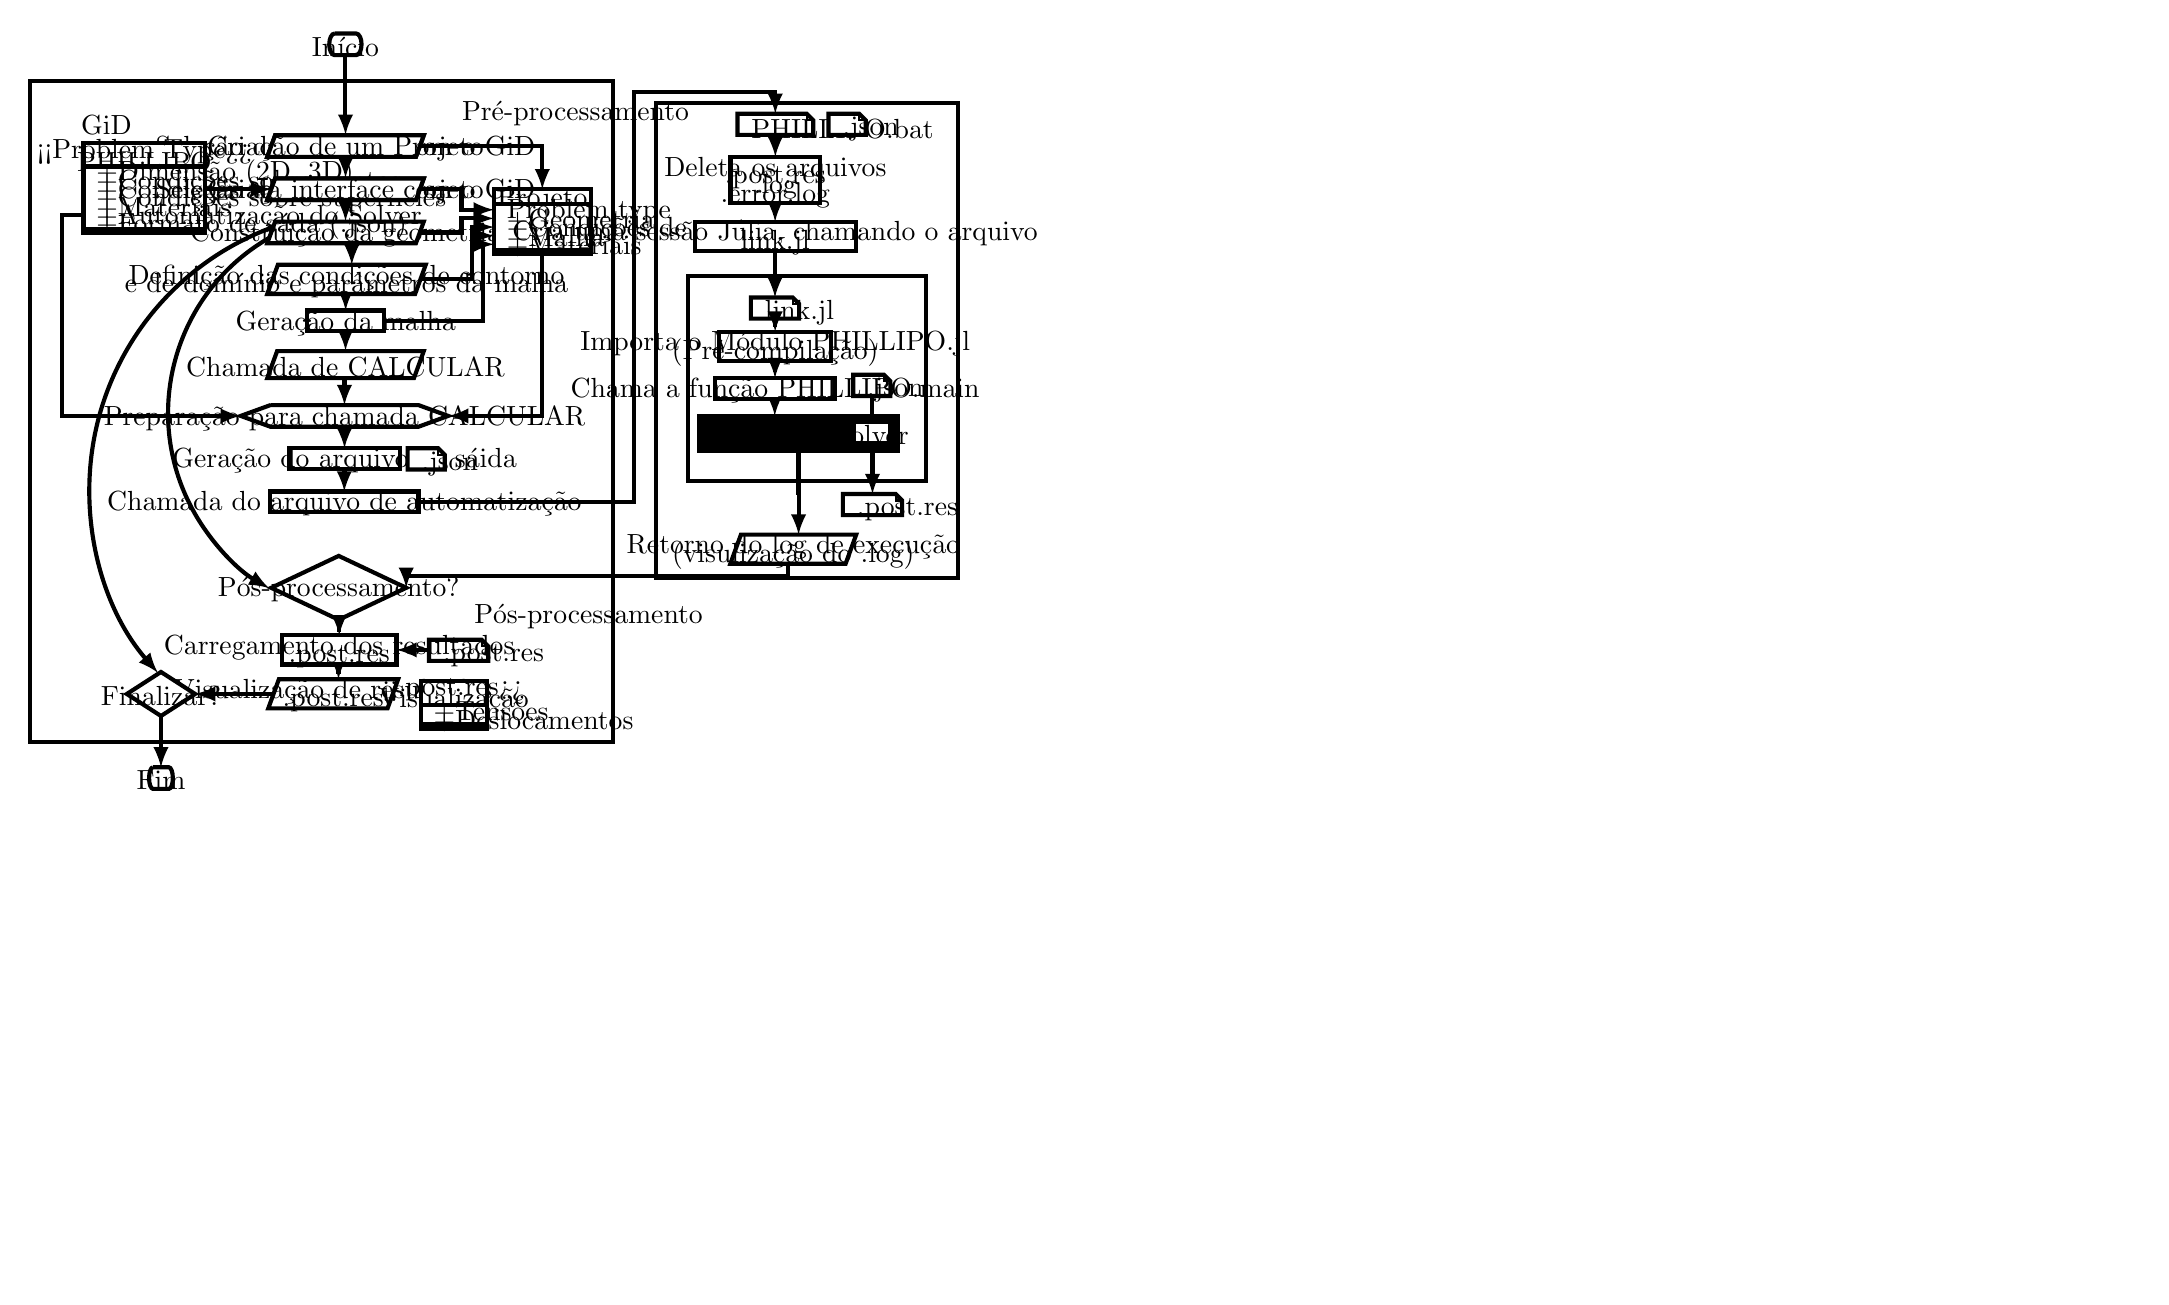
\begin{tikzpicture}
\pgftransformxscale{0.260000}
\pgftransformyscale{-0.260000}
\definecolor{dialinecolor}{rgb}{0.000000, 0.000000, 0.000000}
\pgfsetstrokecolor{dialinecolor}
\definecolor{dialinecolor}{rgb}{1.000000, 1.000000, 1.000000}
\pgfsetfillcolor{dialinecolor}
\pgfsetlinewidth{0.100000\du}
\pgfsetdash{}{0pt}
\pgfsetdash{}{0pt}
\pgfsetmiterjoin
\definecolor{dialinecolor}{rgb}{1.000000, 1.000000, 1.000000}
\pgfsetfillcolor{dialinecolor}
\fill (-57.443080\du,-88.207326\du)--(-57.443080\du,-44.207326\du)--(-29.443080\du,-44.207326\du)--(-29.443080\du,-88.207326\du)--cycle;
\definecolor{dialinecolor}{rgb}{0.000000, 0.000000, 0.000000}
\pgfsetstrokecolor{dialinecolor}
\draw (-57.443080\du,-88.207326\du)--(-57.443080\du,-44.207326\du)--(-29.443080\du,-44.207326\du)--(-29.443080\du,-88.207326\du)--cycle;
\definecolor{dialinecolor}{rgb}{1.000000, 1.000000, 1.000000}
\pgfsetfillcolor{dialinecolor}
\fill (-115.443080\du,-90.207326\du)--(-115.443080\du,-28.976248\du)--(-61.443080\du,-28.976248\du)--(-61.443080\du,-90.207326\du)--cycle;
\pgfsetlinewidth{0.100000\du}
\pgfsetdash{}{0pt}
\pgfsetdash{}{0pt}
\pgfsetmiterjoin
\definecolor{dialinecolor}{rgb}{0.000000, 0.000000, 0.000000}
\pgfsetstrokecolor{dialinecolor}
\draw (-115.443080\du,-90.207326\du)--(-115.443080\du,-28.976248\du)--(-61.443080\du,-28.976248\du)--(-61.443080\du,-90.207326\du)--cycle;
% setfont left to latex
\definecolor{dialinecolor}{rgb}{0.000000, 0.000000, 0.000000}
\pgfsetstrokecolor{dialinecolor}
\node at (-88.443080\du,-59.396787\du){};
\pgfsetlinewidth{0.100000\du}
\pgfsetdash{}{0pt}
\pgfsetdash{}{0pt}
\pgfsetmiterjoin
\pgfsetbuttcap
{
\definecolor{dialinecolor}{rgb}{0.000000, 0.000000, 0.000000}
\pgfsetfillcolor{dialinecolor}
% was here!!!
\pgfsetarrowsend{latex}
{\pgfsetcornersarced{\pgfpoint{0.000000\du}{0.000000\du}}\definecolor{dialinecolor}{rgb}{0.000000, 0.000000, 0.000000}
\pgfsetstrokecolor{dialinecolor}
\draw (-86.180758\du,-67.070540\du)--(-86.180758\du,-67.207326\du)--(-86.193080\du,-67.207326\du)--(-86.193080\du,-65.257405\du);
}}
\pgfsetlinewidth{0.100000\du}
\pgfsetdash{}{0pt}
\pgfsetdash{}{0pt}
\pgfsetbuttcap
\pgfsetmiterjoin
\pgfsetlinewidth{0.100000\du}
\pgfsetbuttcap
\pgfsetmiterjoin
\pgfsetdash{}{0pt}
\definecolor{dialinecolor}{rgb}{1.000000, 1.000000, 1.000000}
\pgfsetfillcolor{dialinecolor}
\pgfpathmoveto{\pgfpoint{-87.202192\du}{-94.636099\du}}
\pgfpathlineto{\pgfpoint{-85.207192\du}{-94.636099\du}}
\pgfpathcurveto{\pgfpoint{-84.931740\du}{-94.636099\du}}{\pgfpoint{-84.708442\du}{-94.188384\du}}{\pgfpoint{-84.708442\du}{-93.636099\du}}
\pgfpathcurveto{\pgfpoint{-84.708442\du}{-93.083814\du}}{\pgfpoint{-84.931740\du}{-92.636099\du}}{\pgfpoint{-85.207192\du}{-92.636099\du}}
\pgfpathlineto{\pgfpoint{-87.202192\du}{-92.636099\du}}
\pgfpathcurveto{\pgfpoint{-87.477644\du}{-92.636099\du}}{\pgfpoint{-87.700942\du}{-93.083814\du}}{\pgfpoint{-87.700942\du}{-93.636099\du}}
\pgfpathcurveto{\pgfpoint{-87.700942\du}{-94.188384\du}}{\pgfpoint{-87.477644\du}{-94.636099\du}}{\pgfpoint{-87.202192\du}{-94.636099\du}}
\pgfusepath{fill}
\definecolor{dialinecolor}{rgb}{0.000000, 0.000000, 0.000000}
\pgfsetstrokecolor{dialinecolor}
\pgfpathmoveto{\pgfpoint{-87.202192\du}{-94.636099\du}}
\pgfpathlineto{\pgfpoint{-85.207192\du}{-94.636099\du}}
\pgfpathcurveto{\pgfpoint{-84.931740\du}{-94.636099\du}}{\pgfpoint{-84.708442\du}{-94.188384\du}}{\pgfpoint{-84.708442\du}{-93.636099\du}}
\pgfpathcurveto{\pgfpoint{-84.708442\du}{-93.083814\du}}{\pgfpoint{-84.931740\du}{-92.636099\du}}{\pgfpoint{-85.207192\du}{-92.636099\du}}
\pgfpathlineto{\pgfpoint{-87.202192\du}{-92.636099\du}}
\pgfpathcurveto{\pgfpoint{-87.477644\du}{-92.636099\du}}{\pgfpoint{-87.700942\du}{-93.083814\du}}{\pgfpoint{-87.700942\du}{-93.636099\du}}
\pgfpathcurveto{\pgfpoint{-87.700942\du}{-94.188384\du}}{\pgfpoint{-87.477644\du}{-94.636099\du}}{\pgfpoint{-87.202192\du}{-94.636099\du}}
\pgfusepath{stroke}
% setfont left to latex
\definecolor{dialinecolor}{rgb}{0.000000, 0.000000, 0.000000}
\pgfsetstrokecolor{dialinecolor}
\node at (-86.204692\du,-93.436099\du){Início};
\definecolor{dialinecolor}{rgb}{1.000000, 1.000000, 1.000000}
\pgfsetfillcolor{dialinecolor}
\fill (-92.715140\du,-85.207326\du)--(-78.943080\du,-85.207326\du)--(-79.671021\du,-83.207326\du)--(-93.443080\du,-83.207326\du)--cycle;
\pgfsetlinewidth{0.100000\du}
\pgfsetdash{}{0pt}
\pgfsetdash{}{0pt}
\pgfsetmiterjoin
\definecolor{dialinecolor}{rgb}{0.000000, 0.000000, 0.000000}
\pgfsetstrokecolor{dialinecolor}
\draw (-92.715140\du,-85.207326\du)--(-78.943080\du,-85.207326\du)--(-79.671021\du,-83.207326\du)--(-93.443080\du,-83.207326\du)--cycle;
% setfont left to latex
\definecolor{dialinecolor}{rgb}{0.000000, 0.000000, 0.000000}
\pgfsetstrokecolor{dialinecolor}
\node at (-86.193080\du,-84.012326\du){Seleção da interface com o GiD};
\definecolor{dialinecolor}{rgb}{1.000000, 1.000000, 1.000000}
\pgfsetfillcolor{dialinecolor}
\fill (-92.715140\du,-77.207326\du)--(-78.943080\du,-77.207326\du)--(-79.671021\du,-75.207326\du)--(-93.443080\du,-75.207326\du)--cycle;
\pgfsetlinewidth{0.100000\du}
\pgfsetdash{}{0pt}
\pgfsetdash{}{0pt}
\pgfsetmiterjoin
\definecolor{dialinecolor}{rgb}{0.000000, 0.000000, 0.000000}
\pgfsetstrokecolor{dialinecolor}
\draw (-92.715140\du,-77.207326\du)--(-78.943080\du,-77.207326\du)--(-79.671021\du,-75.207326\du)--(-93.443080\du,-75.207326\du)--cycle;
% setfont left to latex
\definecolor{dialinecolor}{rgb}{0.000000, 0.000000, 0.000000}
\pgfsetstrokecolor{dialinecolor}
\node at (-86.193080\du,-76.012326\du){Construição da geometria};
% setfont left to latex
\definecolor{dialinecolor}{rgb}{0.000000, 0.000000, 0.000000}
\pgfsetstrokecolor{dialinecolor}
\node[anchor=west] at (-86.443080\du,-57.207326\du){};
% setfont left to latex
\definecolor{dialinecolor}{rgb}{0.000000, 0.000000, 0.000000}
\pgfsetstrokecolor{dialinecolor}
\node[anchor=west] at (-61.223080\du,-73.857326\du){};
\pgfsetlinewidth{0.100000\du}
\pgfsetdash{}{0pt}
\definecolor{dialinecolor}{rgb}{1.000000, 1.000000, 1.000000}
\pgfsetfillcolor{dialinecolor}
\fill (-72.443080\du,-80.207326\du)--(-72.443080\du,-78.807326\du)--(-63.473080\du,-78.807326\du)--(-63.473080\du,-80.207326\du)--cycle;
\definecolor{dialinecolor}{rgb}{0.000000, 0.000000, 0.000000}
\pgfsetstrokecolor{dialinecolor}
\draw (-72.443080\du,-80.207326\du)--(-72.443080\du,-78.807326\du)--(-63.473080\du,-78.807326\du)--(-63.473080\du,-80.207326\du)--cycle;
% setfont left to latex
\definecolor{dialinecolor}{rgb}{0.000000, 0.000000, 0.000000}
\pgfsetstrokecolor{dialinecolor}
\node at (-67.958080\du,-79.257326\du){Projeto};
\definecolor{dialinecolor}{rgb}{1.000000, 1.000000, 1.000000}
\pgfsetfillcolor{dialinecolor}
\fill (-72.443080\du,-78.807326\du)--(-72.443080\du,-74.607326\du)--(-63.473080\du,-74.607326\du)--(-63.473080\du,-78.807326\du)--cycle;
\definecolor{dialinecolor}{rgb}{0.000000, 0.000000, 0.000000}
\pgfsetstrokecolor{dialinecolor}
\draw (-72.443080\du,-78.807326\du)--(-72.443080\du,-74.607326\du)--(-63.473080\du,-74.607326\du)--(-63.473080\du,-78.807326\du)--cycle;
% setfont left to latex
\definecolor{dialinecolor}{rgb}{0.000000, 0.000000, 0.000000}
\pgfsetstrokecolor{dialinecolor}
\node[anchor=west] at (-72.293080\du,-78.107326\du){ Problem type};
% setfont left to latex
\definecolor{dialinecolor}{rgb}{0.000000, 0.000000, 0.000000}
\pgfsetstrokecolor{dialinecolor}
\node[anchor=west] at (-72.293080\du,-77.307326\du){+Geometria};
% setfont left to latex
\definecolor{dialinecolor}{rgb}{0.000000, 0.000000, 0.000000}
\pgfsetstrokecolor{dialinecolor}
\node[anchor=west] at (-72.293080\du,-76.507326\du){+Condições de contorno};
% setfont left to latex
\definecolor{dialinecolor}{rgb}{0.000000, 0.000000, 0.000000}
\pgfsetstrokecolor{dialinecolor}
\node[anchor=west] at (-72.293080\du,-75.707326\du){+Malha};
% setfont left to latex
\definecolor{dialinecolor}{rgb}{0.000000, 0.000000, 0.000000}
\pgfsetstrokecolor{dialinecolor}
\node[anchor=west] at (-72.293080\du,-74.907326\du){+Materiais};
\definecolor{dialinecolor}{rgb}{1.000000, 1.000000, 1.000000}
\pgfsetfillcolor{dialinecolor}
\fill (-72.443080\du,-74.607326\du)--(-72.443080\du,-74.207326\du)--(-63.473080\du,-74.207326\du)--(-63.473080\du,-74.607326\du)--cycle;
\definecolor{dialinecolor}{rgb}{0.000000, 0.000000, 0.000000}
\pgfsetstrokecolor{dialinecolor}
\draw (-72.443080\du,-74.607326\du)--(-72.443080\du,-74.207326\du)--(-63.473080\du,-74.207326\du)--(-63.473080\du,-74.607326\du)--cycle;
\pgfsetlinewidth{0.100000\du}
\pgfsetdash{}{0pt}
\definecolor{dialinecolor}{rgb}{1.000000, 1.000000, 1.000000}
\pgfsetfillcolor{dialinecolor}
\fill (-110.473065\du,-84.516931\du)--(-110.473065\du,-82.316931\du)--(-99.193065\du,-82.316931\du)--(-99.193065\du,-84.516931\du)--cycle;
\definecolor{dialinecolor}{rgb}{0.000000, 0.000000, 0.000000}
\pgfsetstrokecolor{dialinecolor}
\draw (-110.473065\du,-84.516931\du)--(-110.473065\du,-82.316931\du)--(-99.193065\du,-82.316931\du)--(-99.193065\du,-84.516931\du)--cycle;
% setfont left to latex
\definecolor{dialinecolor}{rgb}{0.000000, 0.000000, 0.000000}
\pgfsetstrokecolor{dialinecolor}
\node at (-104.833065\du,-83.716931\du){<<Problem Type>>};
% setfont left to latex
\definecolor{dialinecolor}{rgb}{0.000000, 0.000000, 0.000000}
\pgfsetstrokecolor{dialinecolor}
\node at (-104.833065\du,-82.766931\du){PHILLIPO};
\definecolor{dialinecolor}{rgb}{1.000000, 1.000000, 1.000000}
\pgfsetfillcolor{dialinecolor}
\fill (-110.473065\du,-82.316931\du)--(-110.473065\du,-76.516931\du)--(-99.193065\du,-76.516931\du)--(-99.193065\du,-82.316931\du)--cycle;
\definecolor{dialinecolor}{rgb}{0.000000, 0.000000, 0.000000}
\pgfsetstrokecolor{dialinecolor}
\draw (-110.473065\du,-82.316931\du)--(-110.473065\du,-76.516931\du)--(-99.193065\du,-76.516931\du)--(-99.193065\du,-82.316931\du)--cycle;
% setfont left to latex
\definecolor{dialinecolor}{rgb}{0.000000, 0.000000, 0.000000}
\pgfsetstrokecolor{dialinecolor}
\node[anchor=west] at (-110.323065\du,-81.616931\du){+Dimensão (2D, 3D)};
% setfont left to latex
\definecolor{dialinecolor}{rgb}{0.000000, 0.000000, 0.000000}
\pgfsetstrokecolor{dialinecolor}
\node[anchor=west] at (-110.323065\du,-80.816931\du){+Condições sobre pontos};
% setfont left to latex
\definecolor{dialinecolor}{rgb}{0.000000, 0.000000, 0.000000}
\pgfsetstrokecolor{dialinecolor}
\node[anchor=west] at (-110.323065\du,-80.016931\du){+Condições sobre linhas};
% setfont left to latex
\definecolor{dialinecolor}{rgb}{0.000000, 0.000000, 0.000000}
\pgfsetstrokecolor{dialinecolor}
\node[anchor=west] at (-110.323065\du,-79.216931\du){+Condições sobre superfícies};
% setfont left to latex
\definecolor{dialinecolor}{rgb}{0.000000, 0.000000, 0.000000}
\pgfsetstrokecolor{dialinecolor}
\node[anchor=west] at (-110.323065\du,-78.416931\du){+Materiais};
% setfont left to latex
\definecolor{dialinecolor}{rgb}{0.000000, 0.000000, 0.000000}
\pgfsetstrokecolor{dialinecolor}
\node[anchor=west] at (-110.323065\du,-77.616931\du){+Automatização do Solver};
% setfont left to latex
\definecolor{dialinecolor}{rgb}{0.000000, 0.000000, 0.000000}
\pgfsetstrokecolor{dialinecolor}
\node[anchor=west] at (-110.323065\du,-76.816931\du){+Formato de sáda (.json)};
\definecolor{dialinecolor}{rgb}{1.000000, 1.000000, 1.000000}
\pgfsetfillcolor{dialinecolor}
\fill (-110.473065\du,-76.516931\du)--(-110.473065\du,-76.116931\du)--(-99.193065\du,-76.116931\du)--(-99.193065\du,-76.516931\du)--cycle;
\definecolor{dialinecolor}{rgb}{0.000000, 0.000000, 0.000000}
\pgfsetstrokecolor{dialinecolor}
\draw (-110.473065\du,-76.516931\du)--(-110.473065\du,-76.116931\du)--(-99.193065\du,-76.116931\du)--(-99.193065\du,-76.516931\du)--cycle;
\definecolor{dialinecolor}{rgb}{1.000000, 1.000000, 1.000000}
\pgfsetfillcolor{dialinecolor}
\fill (-92.715140\du,-81.207326\du)--(-78.943080\du,-81.207326\du)--(-79.671021\du,-79.207326\du)--(-93.443080\du,-79.207326\du)--cycle;
\pgfsetlinewidth{0.100000\du}
\pgfsetdash{}{0pt}
\pgfsetdash{}{0pt}
\pgfsetmiterjoin
\definecolor{dialinecolor}{rgb}{0.000000, 0.000000, 0.000000}
\pgfsetstrokecolor{dialinecolor}
\draw (-92.715140\du,-81.207326\du)--(-78.943080\du,-81.207326\du)--(-79.671021\du,-79.207326\du)--(-93.443080\du,-79.207326\du)--cycle;
% setfont left to latex
\definecolor{dialinecolor}{rgb}{0.000000, 0.000000, 0.000000}
\pgfsetstrokecolor{dialinecolor}
\node at (-86.193080\du,-80.012326\du){Criação de um Projeto};
\pgfsetlinewidth{0.100000\du}
\pgfsetdash{}{0pt}
\pgfsetdash{}{0pt}
\pgfsetmiterjoin
\pgfsetbuttcap
{
\definecolor{dialinecolor}{rgb}{0.000000, 0.000000, 0.000000}
\pgfsetfillcolor{dialinecolor}
% was here!!!
\pgfsetarrowsend{latex}
{\pgfsetcornersarced{\pgfpoint{0.000000\du}{0.000000\du}}\definecolor{dialinecolor}{rgb}{0.000000, 0.000000, 0.000000}
\pgfsetstrokecolor{dialinecolor}
\draw (-86.557050\du,-83.207326\du)--(-86.557050\du,-83.207326\du)--(-86.193080\du,-83.207326\du)--(-86.193080\du,-81.256886\du);
}}
\pgfsetlinewidth{0.100000\du}
\pgfsetdash{}{0pt}
\pgfsetdash{}{0pt}
\pgfsetmiterjoin
\pgfsetbuttcap
{
\definecolor{dialinecolor}{rgb}{0.000000, 0.000000, 0.000000}
\pgfsetfillcolor{dialinecolor}
% was here!!!
\pgfsetarrowsend{latex}
{\pgfsetcornersarced{\pgfpoint{0.000000\du}{0.000000\du}}\definecolor{dialinecolor}{rgb}{0.000000, 0.000000, 0.000000}
\pgfsetstrokecolor{dialinecolor}
\draw (-86.557050\du,-79.207326\du)--(-86.557050\du,-79.207326\du)--(-86.193080\du,-79.207326\du)--(-86.193080\du,-77.256886\du);
}}
\pgfsetlinewidth{0.100000\du}
\pgfsetdash{}{0pt}
\pgfsetdash{}{0pt}
\pgfsetmiterjoin
\pgfsetbuttcap
{
\definecolor{dialinecolor}{rgb}{0.000000, 0.000000, 0.000000}
\pgfsetfillcolor{dialinecolor}
% was here!!!
\pgfsetarrowsend{latex}
{\pgfsetcornersarced{\pgfpoint{0.000000\du}{0.000000\du}}\definecolor{dialinecolor}{rgb}{0.000000, 0.000000, 0.000000}
\pgfsetstrokecolor{dialinecolor}
\draw (-86.557050\du,-75.207326\du)--(-86.557050\du,-75.207326\du)--(-85.611684\du,-75.207326\du)--(-85.611684\du,-73.207326\du);
}}
\pgfsetlinewidth{0.100000\du}
\pgfsetdash{}{0pt}
\pgfsetdash{}{0pt}
\pgfsetmiterjoin
\pgfsetbuttcap
{
\definecolor{dialinecolor}{rgb}{0.000000, 0.000000, 0.000000}
\pgfsetfillcolor{dialinecolor}
% was here!!!
\pgfsetarrowsend{latex}
{\pgfsetcornersarced{\pgfpoint{0.000000\du}{0.000000\du}}\definecolor{dialinecolor}{rgb}{0.000000, 0.000000, 0.000000}
\pgfsetstrokecolor{dialinecolor}
\draw (-86.594404\du,-70.507326\du)--(-86.594404\du,-71.078571\du)--(-86.180758\du,-71.078571\du)--(-86.180758\du,-68.970540\du);
}}
\pgfsetlinewidth{0.100000\du}
\pgfsetdash{}{0pt}
\pgfsetdash{}{0pt}
\pgfsetmiterjoin
\pgfsetbuttcap
{
\definecolor{dialinecolor}{rgb}{0.000000, 0.000000, 0.000000}
\pgfsetfillcolor{dialinecolor}
% was here!!!
\pgfsetarrowsend{latex}
{\pgfsetcornersarced{\pgfpoint{0.000000\du}{0.000000\du}}\definecolor{dialinecolor}{rgb}{0.000000, 0.000000, 0.000000}
\pgfsetstrokecolor{dialinecolor}
\draw (-86.193080\du,-84.207326\du)--(-86.193080\du,-84.207326\du)--(-67.958080\du,-84.207326\du)--(-67.958080\du,-80.207326\du);
}}
\definecolor{dialinecolor}{rgb}{1.000000, 1.000000, 1.000000}
\pgfsetfillcolor{dialinecolor}
\fill (-92.715140\du,-85.207326\du)--(-78.943080\du,-85.207326\du)--(-79.671021\du,-83.207326\du)--(-93.443080\du,-83.207326\du)--cycle;
\pgfsetlinewidth{0.100000\du}
\pgfsetdash{}{0pt}
\pgfsetdash{}{0pt}
\pgfsetmiterjoin
\definecolor{dialinecolor}{rgb}{0.000000, 0.000000, 0.000000}
\pgfsetstrokecolor{dialinecolor}
\draw (-92.715140\du,-85.207326\du)--(-78.943080\du,-85.207326\du)--(-79.671021\du,-83.207326\du)--(-93.443080\du,-83.207326\du)--cycle;
% setfont left to latex
\definecolor{dialinecolor}{rgb}{0.000000, 0.000000, 0.000000}
\pgfsetstrokecolor{dialinecolor}
\node at (-86.193080\du,-84.012326\du){Criação de um Projeto};
\definecolor{dialinecolor}{rgb}{1.000000, 1.000000, 1.000000}
\pgfsetfillcolor{dialinecolor}
\fill (-92.715140\du,-81.207326\du)--(-78.943080\du,-81.207326\du)--(-79.671021\du,-79.207326\du)--(-93.443080\du,-79.207326\du)--cycle;
\pgfsetlinewidth{0.100000\du}
\pgfsetdash{}{0pt}
\pgfsetdash{}{0pt}
\pgfsetmiterjoin
\definecolor{dialinecolor}{rgb}{0.000000, 0.000000, 0.000000}
\pgfsetstrokecolor{dialinecolor}
\draw (-92.715140\du,-81.207326\du)--(-78.943080\du,-81.207326\du)--(-79.671021\du,-79.207326\du)--(-93.443080\du,-79.207326\du)--cycle;
% setfont left to latex
\definecolor{dialinecolor}{rgb}{0.000000, 0.000000, 0.000000}
\pgfsetstrokecolor{dialinecolor}
\node at (-86.193080\du,-80.012326\du){Seleção da interface com o GiD};
\pgfsetlinewidth{0.100000\du}
\pgfsetdash{}{0pt}
\pgfsetdash{}{0pt}
\pgfsetmiterjoin
\pgfsetbuttcap
{
\definecolor{dialinecolor}{rgb}{0.000000, 0.000000, 0.000000}
\pgfsetfillcolor{dialinecolor}
% was here!!!
\pgfsetarrowsend{latex}
{\pgfsetcornersarced{\pgfpoint{0.000000\du}{0.000000\du}}\definecolor{dialinecolor}{rgb}{0.000000, 0.000000, 0.000000}
\pgfsetstrokecolor{dialinecolor}
\draw (-79.307050\du,-80.207326\du)--(-75.443080\du,-80.207326\du)--(-75.443080\du,-78.307326\du)--(-72.443080\du,-78.307326\du);
}}
\pgfsetlinewidth{0.100000\du}
\pgfsetdash{}{0pt}
\pgfsetdash{}{0pt}
\pgfsetmiterjoin
\pgfsetbuttcap
{
\definecolor{dialinecolor}{rgb}{0.000000, 0.000000, 0.000000}
\pgfsetfillcolor{dialinecolor}
% was here!!!
\pgfsetarrowsend{latex}
{\pgfsetcornersarced{\pgfpoint{0.000000\du}{0.000000\du}}\definecolor{dialinecolor}{rgb}{0.000000, 0.000000, 0.000000}
\pgfsetstrokecolor{dialinecolor}
\draw (-79.307050\du,-76.207326\du)--(-75.443080\du,-76.207326\du)--(-75.443080\du,-77.507326\du)--(-72.443080\du,-77.507326\du);
}}
\definecolor{dialinecolor}{rgb}{1.000000, 1.000000, 1.000000}
\pgfsetfillcolor{dialinecolor}
\fill (-92.533154\du,-65.207326\du)--(-78.943080\du,-65.207326\du)--(-79.853006\du,-62.707326\du)--(-93.443080\du,-62.707326\du)--cycle;
\pgfsetlinewidth{0.100000\du}
\pgfsetdash{}{0pt}
\pgfsetdash{}{0pt}
\pgfsetmiterjoin
\definecolor{dialinecolor}{rgb}{0.000000, 0.000000, 0.000000}
\pgfsetstrokecolor{dialinecolor}
\draw (-92.533154\du,-65.207326\du)--(-78.943080\du,-65.207326\du)--(-79.853006\du,-62.707326\du)--(-93.443080\du,-62.707326\du)--cycle;
% setfont left to latex
\definecolor{dialinecolor}{rgb}{0.000000, 0.000000, 0.000000}
\pgfsetstrokecolor{dialinecolor}
\node at (-86.193080\du,-63.762326\du){Chamada de CALCULAR};
\definecolor{dialinecolor}{rgb}{1.000000, 1.000000, 1.000000}
\pgfsetfillcolor{dialinecolor}
\fill (-92.460360\du,-73.207326\du)--(-78.763008\du,-73.207326\du)--(-79.745728\du,-70.507326\du)--(-93.443080\du,-70.507326\du)--cycle;
\pgfsetlinewidth{0.100000\du}
\pgfsetdash{}{0pt}
\pgfsetdash{}{0pt}
\pgfsetmiterjoin
\definecolor{dialinecolor}{rgb}{0.000000, 0.000000, 0.000000}
\pgfsetstrokecolor{dialinecolor}
\draw (-92.460360\du,-73.207326\du)--(-78.763008\du,-73.207326\du)--(-79.745728\du,-70.507326\du)--(-93.443080\du,-70.507326\du)--cycle;
% setfont left to latex
\definecolor{dialinecolor}{rgb}{0.000000, 0.000000, 0.000000}
\pgfsetstrokecolor{dialinecolor}
\node at (-86.103044\du,-72.062326\du){Definição das condições de contorno};
% setfont left to latex
\definecolor{dialinecolor}{rgb}{0.000000, 0.000000, 0.000000}
\pgfsetstrokecolor{dialinecolor}
\node at (-86.103044\du,-71.262326\du){e de domínio e parâmetros da malha};
\pgfsetlinewidth{0.100000\du}
\pgfsetdash{}{0pt}
\pgfsetdash{}{0pt}
\pgfsetmiterjoin
\pgfsetbuttcap
{
\definecolor{dialinecolor}{rgb}{0.000000, 0.000000, 0.000000}
\pgfsetfillcolor{dialinecolor}
% was here!!!
\pgfsetarrowsend{latex}
{\pgfsetcornersarced{\pgfpoint{0.000000\du}{0.000000\du}}\definecolor{dialinecolor}{rgb}{0.000000, 0.000000, 0.000000}
\pgfsetstrokecolor{dialinecolor}
\draw (-79.254368\du,-71.857326\du)--(-74.443080\du,-71.857326\du)--(-74.443080\du,-76.707326\du)--(-72.443080\du,-76.707326\du);
}}
\pgfsetlinewidth{0.100000\du}
\pgfsetdash{}{0pt}
\pgfsetdash{}{0pt}
\pgfsetmiterjoin
\pgfsetbuttcap
{
\definecolor{dialinecolor}{rgb}{0.000000, 0.000000, 0.000000}
\pgfsetfillcolor{dialinecolor}
% was here!!!
\pgfsetarrowsend{latex}
{\pgfsetcornersarced{\pgfpoint{0.000000\du}{0.000000\du}}\definecolor{dialinecolor}{rgb}{0.000000, 0.000000, 0.000000}
\pgfsetstrokecolor{dialinecolor}
\draw (-86.648043\du,-62.707326\du)--(-86.648043\du,-62.707326\du)--(-86.291080\du,-62.707326\du)--(-86.291080\du,-60.207326\du);
}}
\pgfsetlinewidth{0.100000\du}
\pgfsetdash{}{0pt}
\pgfsetdash{}{0pt}
\pgfsetmiterjoin
\pgfsetbuttcap
{
\definecolor{dialinecolor}{rgb}{0.000000, 0.000000, 0.000000}
\pgfsetfillcolor{dialinecolor}
% was here!!!
\pgfsetarrowsend{latex}
{\pgfsetcornersarced{\pgfpoint{0.000000\du}{0.000000\du}}\definecolor{dialinecolor}{rgb}{0.000000, 0.000000, 0.000000}
\pgfsetstrokecolor{dialinecolor}
\draw (-82.592008\du,-68.020540\du)--(-73.443080\du,-68.020540\du)--(-73.443080\du,-75.107326\du)--(-72.443080\du,-75.107326\du);
}}
\pgfsetlinewidth{0.100000\du}
\pgfsetdash{}{0pt}
\pgfsetdash{}{0pt}
\pgfsetmiterjoin
\pgfsetbuttcap
{
\definecolor{dialinecolor}{rgb}{0.000000, 0.000000, 0.000000}
\pgfsetfillcolor{dialinecolor}
% was here!!!
\pgfsetarrowsend{latex}
{\pgfsetcornersarced{\pgfpoint{0.000000\du}{0.000000\du}}\definecolor{dialinecolor}{rgb}{0.000000, 0.000000, 0.000000}
\pgfsetstrokecolor{dialinecolor}
\draw (-74.443080\du,-75.807326\du)--(-74.443080\du,-75.807326\du)--(-74.443080\du,-75.907326\du)--(-72.443080\du,-75.907326\du);
}}
\pgfsetlinewidth{0.100000\du}
\pgfsetdash{}{0pt}
\pgfsetdash{}{0pt}
\pgfsetmiterjoin
\pgfsetbuttcap
{
\definecolor{dialinecolor}{rgb}{0.000000, 0.000000, 0.000000}
\pgfsetfillcolor{dialinecolor}
% was here!!!
\pgfsetarrowsend{latex}
{\pgfsetcornersarced{\pgfpoint{0.000000\du}{0.000000\du}}\definecolor{dialinecolor}{rgb}{0.000000, 0.000000, 0.000000}
\pgfsetstrokecolor{dialinecolor}
\draw (-67.958080\du,-74.207326\du)--(-67.958080\du,-59.207326\du)--(-76.680080\du,-59.207326\du);
}}
\pgfsetlinewidth{0.100000\du}
\pgfsetdash{}{0pt}
\pgfsetdash{}{0pt}
\pgfsetmiterjoin
\pgfsetbuttcap
{
\definecolor{dialinecolor}{rgb}{0.000000, 0.000000, 0.000000}
\pgfsetfillcolor{dialinecolor}
% was here!!!
\pgfsetarrowsend{latex}
{\pgfsetcornersarced{\pgfpoint{0.000000\du}{0.000000\du}}\definecolor{dialinecolor}{rgb}{0.000000, 0.000000, 0.000000}
\pgfsetstrokecolor{dialinecolor}
\draw (-99.193065\du,-80.216931\du)--(-94.371095\du,-80.216931\du)--(-94.371095\du,-80.207326\du)--(-93.079110\du,-80.207326\du);
}}
\pgfsetlinewidth{0.100000\du}
\pgfsetdash{}{0pt}
\pgfsetdash{}{0pt}
\pgfsetmiterjoin
\pgfsetbuttcap
{
\definecolor{dialinecolor}{rgb}{0.000000, 0.000000, 0.000000}
\pgfsetfillcolor{dialinecolor}
% was here!!!
\pgfsetarrowsend{latex}
{\pgfsetcornersarced{\pgfpoint{0.000000\du}{0.000000\du}}\definecolor{dialinecolor}{rgb}{0.000000, 0.000000, 0.000000}
\pgfsetstrokecolor{dialinecolor}
\draw (-86.204692\du,-92.636099\du)--(-86.204692\du,-86.732454\du)--(-86.193080\du,-86.732454\du)--(-86.193080\du,-85.255353\du);
}}
\pgfsetlinewidth{0.100000\du}
\pgfsetdash{}{0pt}
\pgfsetdash{}{0pt}
\pgfsetmiterjoin
\pgfsetbuttcap
{
\definecolor{dialinecolor}{rgb}{0.000000, 0.000000, 0.000000}
\pgfsetfillcolor{dialinecolor}
% was here!!!
\pgfsetarrowsend{latex}
{\pgfsetcornersarced{\pgfpoint{0.000000\du}{0.000000\du}}\definecolor{dialinecolor}{rgb}{0.000000, 0.000000, 0.000000}
\pgfsetstrokecolor{dialinecolor}
\draw (-110.473065\du,-77.816931\du)--(-112.443080\du,-77.816931\du)--(-112.443080\du,-59.207326\du)--(-95.900457\du,-59.207326\du);
}}
\definecolor{dialinecolor}{rgb}{1.000000, 1.000000, 1.000000}
\pgfsetfillcolor{dialinecolor}
\fill (-89.769508\du,-68.970540\du)--(-89.769508\du,-67.070540\du)--(-82.592008\du,-67.070540\du)--(-82.592008\du,-68.970540\du)--cycle;
\pgfsetlinewidth{0.100000\du}
\pgfsetdash{}{0pt}
\pgfsetdash{}{0pt}
\pgfsetmiterjoin
\definecolor{dialinecolor}{rgb}{0.000000, 0.000000, 0.000000}
\pgfsetstrokecolor{dialinecolor}
\draw (-89.769508\du,-68.970540\du)--(-89.769508\du,-67.070540\du)--(-82.592008\du,-67.070540\du)--(-82.592008\du,-68.970540\du)--cycle;
% setfont left to latex
\definecolor{dialinecolor}{rgb}{0.000000, 0.000000, 0.000000}
\pgfsetstrokecolor{dialinecolor}
\node at (-86.180758\du,-67.825540\du){Geração da malha};
\definecolor{dialinecolor}{rgb}{1.000000, 1.000000, 1.000000}
\pgfsetfillcolor{dialinecolor}
\fill (-91.443080\du,-56.207326\du)--(-91.443080\du,-54.307326\du)--(-81.128080\du,-54.307326\du)--(-81.128080\du,-56.207326\du)--cycle;
\pgfsetlinewidth{0.100000\du}
\pgfsetdash{}{0pt}
\pgfsetdash{}{0pt}
\pgfsetmiterjoin
\definecolor{dialinecolor}{rgb}{0.000000, 0.000000, 0.000000}
\pgfsetstrokecolor{dialinecolor}
\draw (-91.443080\du,-56.207326\du)--(-91.443080\du,-54.307326\du)--(-81.128080\du,-54.307326\du)--(-81.128080\du,-56.207326\du)--cycle;
% setfont left to latex
\definecolor{dialinecolor}{rgb}{0.000000, 0.000000, 0.000000}
\pgfsetstrokecolor{dialinecolor}
\node at (-86.285580\du,-55.062326\du){Geração do arquivo de sáida};
\definecolor{dialinecolor}{rgb}{1.000000, 1.000000, 1.000000}
\pgfsetfillcolor{dialinecolor}
\fill (-93.173218\du,-52.207326\du)--(-93.173218\du,-50.307326\du)--(-79.435718\du,-50.307326\du)--(-79.435718\du,-52.207326\du)--cycle;
\pgfsetlinewidth{0.100000\du}
\pgfsetdash{}{0pt}
\pgfsetdash{}{0pt}
\pgfsetmiterjoin
\definecolor{dialinecolor}{rgb}{0.000000, 0.000000, 0.000000}
\pgfsetstrokecolor{dialinecolor}
\draw (-93.173218\du,-52.207326\du)--(-93.173218\du,-50.307326\du)--(-79.435718\du,-50.307326\du)--(-79.435718\du,-52.207326\du)--cycle;
% setfont left to latex
\definecolor{dialinecolor}{rgb}{0.000000, 0.000000, 0.000000}
\pgfsetstrokecolor{dialinecolor}
\node at (-86.304468\du,-51.062326\du){Chamada do arquivo de automatização};
\pgfsetlinewidth{0.100000\du}
\pgfsetdash{}{0pt}
\pgfsetdash{}{0pt}
\pgfsetmiterjoin
\pgfsetbuttcap
{
\definecolor{dialinecolor}{rgb}{0.000000, 0.000000, 0.000000}
\pgfsetfillcolor{dialinecolor}
% was here!!!
\pgfsetarrowsend{latex}
{\pgfsetcornersarced{\pgfpoint{0.000000\du}{0.000000\du}}\definecolor{dialinecolor}{rgb}{0.000000, 0.000000, 0.000000}
\pgfsetstrokecolor{dialinecolor}
\draw (-86.285580\du,-54.307326\du)--(-86.285580\du,-53.257326\du)--(-86.304468\du,-53.257326\du)--(-86.304468\du,-52.207326\du);
}}
\pgfsetlinewidth{0.100000\du}
\pgfsetdash{}{0pt}
\pgfsetdash{}{0pt}
\pgfsetmiterjoin
\pgfsetbuttcap
{
\definecolor{dialinecolor}{rgb}{0.000000, 0.000000, 0.000000}
\pgfsetfillcolor{dialinecolor}
% was here!!!
\pgfsetarrowsend{latex}
{\pgfsetcornersarced{\pgfpoint{0.000000\du}{0.000000\du}}\definecolor{dialinecolor}{rgb}{0.000000, 0.000000, 0.000000}
\pgfsetstrokecolor{dialinecolor}
\draw (-89.723580\du,-58.207326\du)--(-89.723580\du,-59.207326\du)--(-86.285580\du,-59.207326\du)--(-86.285580\du,-56.207326\du);
}}
\pgfsetlinewidth{0.100000\du}
\pgfsetdash{}{0pt}
\pgfsetdash{}{0pt}
\pgfsetbuttcap
\pgfsetmiterjoin
\pgfsetlinewidth{0.100000\du}
\pgfsetbuttcap
\pgfsetmiterjoin
\pgfsetdash{}{0pt}
\definecolor{dialinecolor}{rgb}{1.000000, 1.000000, 1.000000}
\pgfsetfillcolor{dialinecolor}
\pgfpathmoveto{\pgfpoint{-93.156080\du}{-60.207326\du}}
\pgfpathlineto{\pgfpoint{-79.426080\du}{-60.207326\du}}
\pgfpathlineto{\pgfpoint{-76.680080\du}{-59.207326\du}}
\pgfpathlineto{\pgfpoint{-79.426080\du}{-58.207326\du}}
\pgfpathlineto{\pgfpoint{-93.156080\du}{-58.207326\du}}
\pgfpathlineto{\pgfpoint{-95.902080\du}{-59.207326\du}}
\pgfpathlineto{\pgfpoint{-93.156080\du}{-60.207326\du}}
\pgfusepath{fill}
\definecolor{dialinecolor}{rgb}{0.000000, 0.000000, 0.000000}
\pgfsetstrokecolor{dialinecolor}
\pgfpathmoveto{\pgfpoint{-93.156080\du}{-60.207326\du}}
\pgfpathlineto{\pgfpoint{-79.426080\du}{-60.207326\du}}
\pgfpathlineto{\pgfpoint{-76.680080\du}{-59.207326\du}}
\pgfpathlineto{\pgfpoint{-79.426080\du}{-58.207326\du}}
\pgfpathlineto{\pgfpoint{-93.156080\du}{-58.207326\du}}
\pgfpathlineto{\pgfpoint{-95.902080\du}{-59.207326\du}}
\pgfpathlineto{\pgfpoint{-93.156080\du}{-60.207326\du}}
\pgfusepath{stroke}
% setfont left to latex
\definecolor{dialinecolor}{rgb}{0.000000, 0.000000, 0.000000}
\pgfsetstrokecolor{dialinecolor}
\node at (-86.291080\du,-59.007326\du){Preparação para chamada CALCULAR};
% setfont left to latex
\definecolor{dialinecolor}{rgb}{0.000000, 0.000000, 0.000000}
\pgfsetstrokecolor{dialinecolor}
\node[anchor=west] at (-88.443080\du,-59.591787\du){};
% setfont left to latex
\definecolor{dialinecolor}{rgb}{0.000000, 0.000000, 0.000000}
\pgfsetstrokecolor{dialinecolor}
\node[anchor=west] at (-88.443080\du,-59.591787\du){};
% setfont left to latex
\definecolor{dialinecolor}{rgb}{0.000000, 0.000000, 1.000000}
\pgfsetstrokecolor{dialinecolor}
\node[anchor=west] at (-111.742197\du,-86.119838\du){GiD};
\pgfsetlinewidth{0.100000\du}
\pgfsetdash{}{0pt}
\definecolor{dialinecolor}{rgb}{1.000000, 1.000000, 1.000000}
\pgfsetfillcolor{dialinecolor}
\fill (-49.881469\du,-87.207326\du)--(-43.461469\du,-87.207326\du)--(-42.861469\du,-86.607326\du)--(-42.861469\du,-85.248992\du)--(-49.881469\du,-85.248992\du)--cycle;
\definecolor{dialinecolor}{rgb}{0.000000, 0.000000, 0.000000}
\pgfsetstrokecolor{dialinecolor}
\draw (-49.881469\du,-87.207326\du)--(-43.461469\du,-87.207326\du)--(-42.861469\du,-86.607326\du)--(-42.861469\du,-85.248992\du)--(-49.881469\du,-85.248992\du)--cycle;
\pgfsetlinewidth{0.050000\du}
\definecolor{dialinecolor}{rgb}{0.000000, 0.000000, 0.000000}
\pgfsetstrokecolor{dialinecolor}
\draw (-43.461469\du,-87.207326\du)--(-43.461469\du,-86.607326\du)--(-42.861469\du,-86.607326\du);
% setfont left to latex
\definecolor{dialinecolor}{rgb}{0.000000, 0.000000, 0.000000}
\pgfsetstrokecolor{dialinecolor}
\node[anchor=west] at (-49.531469\du,-85.769826\du){PHILLIPO.bat};
\pgfsetlinewidth{0.100000\du}
\pgfsetdash{}{0pt}
\pgfsetdash{}{0pt}
\pgfsetmiterjoin
\pgfsetbuttcap
{
\definecolor{dialinecolor}{rgb}{0.000000, 0.000000, 0.000000}
\pgfsetfillcolor{dialinecolor}
% was here!!!
\pgfsetarrowsend{latex}
{\pgfsetcornersarced{\pgfpoint{0.000000\du}{0.000000\du}}\definecolor{dialinecolor}{rgb}{0.000000, 0.000000, 0.000000}
\pgfsetstrokecolor{dialinecolor}
\draw (-79.435718\du,-51.257326\du)--(-59.443080\du,-51.257326\du)--(-59.443080\du,-89.207326\du)--(-46.371469\du,-89.207326\du)--(-46.371469\du,-87.207326\du);
}}
\definecolor{dialinecolor}{rgb}{1.000000, 1.000000, 1.000000}
\pgfsetfillcolor{dialinecolor}
\fill (-50.516650\du,-83.207326\du)--(-50.516650\du,-78.907326\du)--(-42.221650\du,-78.907326\du)--(-42.221650\du,-83.207326\du)--cycle;
\pgfsetlinewidth{0.100000\du}
\pgfsetdash{}{0pt}
\pgfsetdash{}{0pt}
\pgfsetmiterjoin
\definecolor{dialinecolor}{rgb}{0.000000, 0.000000, 0.000000}
\pgfsetstrokecolor{dialinecolor}
\draw (-50.516650\du,-83.207326\du)--(-50.516650\du,-78.907326\du)--(-42.221650\du,-78.907326\du)--(-42.221650\du,-83.207326\du)--cycle;
% setfont left to latex
\definecolor{dialinecolor}{rgb}{0.000000, 0.000000, 0.000000}
\pgfsetstrokecolor{dialinecolor}
\node at (-46.369150\du,-82.062326\du){Deleta os arquivos };
% setfont left to latex
\definecolor{dialinecolor}{rgb}{0.000000, 0.000000, 0.000000}
\pgfsetstrokecolor{dialinecolor}
\node at (-46.369150\du,-81.262326\du){.post.res};
% setfont left to latex
\definecolor{dialinecolor}{rgb}{0.000000, 0.000000, 0.000000}
\pgfsetstrokecolor{dialinecolor}
\node at (-46.369150\du,-80.462326\du){.log};
% setfont left to latex
\definecolor{dialinecolor}{rgb}{0.000000, 0.000000, 0.000000}
\pgfsetstrokecolor{dialinecolor}
\node at (-46.369150\du,-79.662326\du){.error.log};
% setfont left to latex
\definecolor{dialinecolor}{rgb}{0.000000, 0.000000, 0.000000}
\pgfsetstrokecolor{dialinecolor}
\node[anchor=west] at (-76.443080\du,-87.207326\du){Pré-processamento};
% setfont left to latex
\definecolor{dialinecolor}{rgb}{0.000000, 0.000000, 0.000000}
\pgfsetstrokecolor{dialinecolor}
\node[anchor=west] at (-75.313033\du,-40.589275\du){Pós-processamento};
\definecolor{dialinecolor}{rgb}{1.000000, 1.000000, 1.000000}
\pgfsetfillcolor{dialinecolor}
\fill (-53.847714\du,-77.207326\du)--(-53.847714\du,-74.507326\du)--(-38.930214\du,-74.507326\du)--(-38.930214\du,-77.207326\du)--cycle;
\pgfsetlinewidth{0.100000\du}
\pgfsetdash{}{0pt}
\pgfsetdash{}{0pt}
\pgfsetmiterjoin
\definecolor{dialinecolor}{rgb}{0.000000, 0.000000, 0.000000}
\pgfsetstrokecolor{dialinecolor}
\draw (-53.847714\du,-77.207326\du)--(-53.847714\du,-74.507326\du)--(-38.930214\du,-74.507326\du)--(-38.930214\du,-77.207326\du)--cycle;
% setfont left to latex
\definecolor{dialinecolor}{rgb}{0.000000, 0.000000, 0.000000}
\pgfsetstrokecolor{dialinecolor}
\node at (-46.388964\du,-76.062326\du){Cria uma sessão Julia, chamando o arquivo};
% setfont left to latex
\definecolor{dialinecolor}{rgb}{0.000000, 0.000000, 0.000000}
\pgfsetstrokecolor{dialinecolor}
\node at (-46.388964\du,-75.262326\du){link.jl};
\definecolor{dialinecolor}{rgb}{1.000000, 1.000000, 1.000000}
\pgfsetfillcolor{dialinecolor}
\fill (-54.443080\du,-72.207326\du)--(-54.443080\du,-53.207326\du)--(-32.443080\du,-53.207326\du)--(-32.443080\du,-72.207326\du)--cycle;
\pgfsetlinewidth{0.100000\du}
\pgfsetdash{}{0pt}
\pgfsetdash{}{0pt}
\pgfsetmiterjoin
\definecolor{dialinecolor}{rgb}{0.000000, 0.000000, 0.000000}
\pgfsetstrokecolor{dialinecolor}
\draw (-54.443080\du,-72.207326\du)--(-54.443080\du,-53.207326\du)--(-32.443080\du,-53.207326\du)--(-32.443080\du,-72.207326\du)--cycle;
% setfont left to latex
\definecolor{dialinecolor}{rgb}{0.000000, 0.000000, 0.000000}
\pgfsetstrokecolor{dialinecolor}
\node at (-43.443080\du,-62.512326\du){};
% image rendering not supported\pgfsetlinewidth{0.100000\du}
\pgfsetdash{}{0pt}
\definecolor{dialinecolor}{rgb}{1.000000, 1.000000, 1.000000}
\pgfsetfillcolor{dialinecolor}
\fill (-48.633896\du,-70.183474\du)--(-44.763896\du,-70.183474\du)--(-44.163896\du,-69.583474\du)--(-44.163896\du,-68.225140\du)--(-48.633896\du,-68.225140\du)--cycle;
\definecolor{dialinecolor}{rgb}{0.000000, 0.000000, 0.000000}
\pgfsetstrokecolor{dialinecolor}
\draw (-48.633896\du,-70.183474\du)--(-44.763896\du,-70.183474\du)--(-44.163896\du,-69.583474\du)--(-44.163896\du,-68.225140\du)--(-48.633896\du,-68.225140\du)--cycle;
\pgfsetlinewidth{0.050000\du}
\definecolor{dialinecolor}{rgb}{0.000000, 0.000000, 0.000000}
\pgfsetstrokecolor{dialinecolor}
\draw (-44.763896\du,-70.183474\du)--(-44.763896\du,-69.583474\du)--(-44.163896\du,-69.583474\du);
% setfont left to latex
\definecolor{dialinecolor}{rgb}{0.000000, 0.000000, 0.000000}
\pgfsetstrokecolor{dialinecolor}
\node[anchor=west] at (-48.283896\du,-68.745974\du){link.jl};
\pgfsetlinewidth{0.100000\du}
\pgfsetdash{}{0pt}
\definecolor{dialinecolor}{rgb}{1.000000, 1.000000, 1.000000}
\pgfsetfillcolor{dialinecolor}
\fill (-41.443080\du,-87.207326\du)--(-38.593080\du,-87.207326\du)--(-37.993080\du,-86.607326\du)--(-37.993080\du,-85.248992\du)--(-41.443080\du,-85.248992\du)--cycle;
\definecolor{dialinecolor}{rgb}{0.000000, 0.000000, 0.000000}
\pgfsetstrokecolor{dialinecolor}
\draw (-41.443080\du,-87.207326\du)--(-38.593080\du,-87.207326\du)--(-37.993080\du,-86.607326\du)--(-37.993080\du,-85.248992\du)--(-41.443080\du,-85.248992\du)--cycle;
\pgfsetlinewidth{0.050000\du}
\definecolor{dialinecolor}{rgb}{0.000000, 0.000000, 0.000000}
\pgfsetstrokecolor{dialinecolor}
\draw (-38.593080\du,-87.207326\du)--(-38.593080\du,-86.607326\du)--(-37.993080\du,-86.607326\du);
% setfont left to latex
\definecolor{dialinecolor}{rgb}{0.000000, 0.000000, 0.000000}
\pgfsetstrokecolor{dialinecolor}
\node[anchor=west] at (-41.093080\du,-85.769826\du){.json};
\definecolor{dialinecolor}{rgb}{1.000000, 1.000000, 1.000000}
\pgfsetfillcolor{dialinecolor}
\fill (-51.562340\du,-67.016510\du)--(-51.562340\du,-64.316510\du)--(-41.207340\du,-64.316510\du)--(-41.207340\du,-67.016510\du)--cycle;
\pgfsetlinewidth{0.100000\du}
\pgfsetdash{}{0pt}
\pgfsetdash{}{0pt}
\pgfsetmiterjoin
\definecolor{dialinecolor}{rgb}{0.000000, 0.000000, 0.000000}
\pgfsetstrokecolor{dialinecolor}
\draw (-51.562340\du,-67.016510\du)--(-51.562340\du,-64.316510\du)--(-41.207340\du,-64.316510\du)--(-41.207340\du,-67.016510\du)--cycle;
% setfont left to latex
\definecolor{dialinecolor}{rgb}{0.000000, 0.000000, 0.000000}
\pgfsetstrokecolor{dialinecolor}
\node at (-46.384840\du,-65.871510\du){Importa o Módulo PHILLIPO.jl};
% setfont left to latex
\definecolor{dialinecolor}{rgb}{0.000000, 0.000000, 0.000000}
\pgfsetstrokecolor{dialinecolor}
\node at (-46.384840\du,-65.071510\du){(Pré-compilação)};
\pgfsetlinewidth{0.100000\du}
\pgfsetdash{}{0pt}
\definecolor{dialinecolor}{rgb}{1.000000, 1.000000, 1.000000}
\pgfsetfillcolor{dialinecolor}
\fill (-80.443080\du,-56.207326\du)--(-77.593080\du,-56.207326\du)--(-76.993080\du,-55.607326\du)--(-76.993080\du,-54.248992\du)--(-80.443080\du,-54.248992\du)--cycle;
\definecolor{dialinecolor}{rgb}{0.000000, 0.000000, 0.000000}
\pgfsetstrokecolor{dialinecolor}
\draw (-80.443080\du,-56.207326\du)--(-77.593080\du,-56.207326\du)--(-76.993080\du,-55.607326\du)--(-76.993080\du,-54.248992\du)--(-80.443080\du,-54.248992\du)--cycle;
\pgfsetlinewidth{0.050000\du}
\definecolor{dialinecolor}{rgb}{0.000000, 0.000000, 0.000000}
\pgfsetstrokecolor{dialinecolor}
\draw (-77.593080\du,-56.207326\du)--(-77.593080\du,-55.607326\du)--(-76.993080\du,-55.607326\du);
% setfont left to latex
\definecolor{dialinecolor}{rgb}{0.000000, 0.000000, 0.000000}
\pgfsetstrokecolor{dialinecolor}
\node[anchor=west] at (-80.093080\du,-54.769826\du){.json};
\definecolor{dialinecolor}{rgb}{0.000000, 0.000000, 0.000000}
\pgfsetfillcolor{dialinecolor}
\fill (-53.443080\du,-59.207326\du)--(-53.443080\du,-55.990659\du)--(-35.003080\du,-55.990659\du)--(-35.003080\du,-59.207326\du)--cycle;
\pgfsetlinewidth{0.100000\du}
\pgfsetdash{}{0pt}
\pgfsetdash{}{0pt}
\pgfsetmiterjoin
\definecolor{dialinecolor}{rgb}{0.000000, 0.000000, 0.000000}
\pgfsetstrokecolor{dialinecolor}
\draw (-53.443080\du,-59.207326\du)--(-53.443080\du,-55.990659\du)--(-35.003080\du,-55.990659\du)--(-35.003080\du,-59.207326\du)--cycle;
% setfont left to latex
\definecolor{dialinecolor}{rgb}{1.000000, 1.000000, 1.000000}
\pgfsetstrokecolor{dialinecolor}
\node at (-44.223080\du,-57.087326\du){PHILLIPO.main    };
\pgfsetlinewidth{0.100000\du}
\pgfsetdash{}{0pt}
\pgfsetdash{}{0pt}
\pgfsetmiterjoin
\pgfsetbuttcap
{
\definecolor{dialinecolor}{rgb}{0.000000, 0.000000, 0.000000}
\pgfsetfillcolor{dialinecolor}
% was here!!!
\pgfsetarrowsend{latex}
{\pgfsetcornersarced{\pgfpoint{0.000000\du}{0.000000\du}}\definecolor{dialinecolor}{rgb}{0.000000, 0.000000, 0.000000}
\pgfsetstrokecolor{dialinecolor}
\draw (-46.371469\du,-85.248992\du)--(-46.371469\du,-84.228159\du)--(-46.369150\du,-84.228159\du)--(-46.369150\du,-83.207326\du);
}}
\pgfsetlinewidth{0.100000\du}
\pgfsetdash{}{0pt}
\pgfsetdash{}{0pt}
\pgfsetmiterjoin
\pgfsetbuttcap
{
\definecolor{dialinecolor}{rgb}{0.000000, 0.000000, 0.000000}
\pgfsetfillcolor{dialinecolor}
% was here!!!
\pgfsetarrowsend{latex}
{\pgfsetcornersarced{\pgfpoint{0.000000\du}{0.000000\du}}\definecolor{dialinecolor}{rgb}{0.000000, 0.000000, 0.000000}
\pgfsetstrokecolor{dialinecolor}
\draw (-46.369150\du,-78.907326\du)--(-46.369150\du,-78.057326\du)--(-46.388964\du,-78.057326\du)--(-46.388964\du,-77.207326\du);
}}
\pgfsetlinewidth{0.100000\du}
\pgfsetdash{}{0pt}
\pgfsetdash{}{0pt}
\pgfsetmiterjoin
\pgfsetbuttcap
{
\definecolor{dialinecolor}{rgb}{0.000000, 0.000000, 0.000000}
\pgfsetfillcolor{dialinecolor}
% was here!!!
\pgfsetarrowsend{latex}
{\pgfsetcornersarced{\pgfpoint{0.000000\du}{0.000000\du}}\definecolor{dialinecolor}{rgb}{0.000000, 0.000000, 0.000000}
\pgfsetstrokecolor{dialinecolor}
\draw (-46.388964\du,-74.507326\du)--(-46.388964\du,-72.345400\du)--(-46.398896\du,-72.345400\du)--(-46.398896\du,-70.183474\du);
}}
\pgfsetlinewidth{0.100000\du}
\pgfsetdash{}{0pt}
\pgfsetdash{}{0pt}
\pgfsetmiterjoin
\pgfsetbuttcap
{
\definecolor{dialinecolor}{rgb}{0.000000, 0.000000, 0.000000}
\pgfsetfillcolor{dialinecolor}
% was here!!!
\pgfsetarrowsend{latex}
{\pgfsetcornersarced{\pgfpoint{0.000000\du}{0.000000\du}}\definecolor{dialinecolor}{rgb}{0.000000, 0.000000, 0.000000}
\pgfsetstrokecolor{dialinecolor}
\draw (-46.398896\du,-68.225140\du)--(-46.398896\du,-67.620825\du)--(-46.384840\du,-67.620825\du)--(-46.384840\du,-67.016510\du);
}}
\pgfsetlinewidth{0.100000\du}
\pgfsetdash{}{0pt}
\pgfsetdash{}{0pt}
\pgfsetmiterjoin
\pgfsetbuttcap
{
\definecolor{dialinecolor}{rgb}{0.000000, 0.000000, 0.000000}
\pgfsetfillcolor{dialinecolor}
% was here!!!
\pgfsetarrowsend{latex}
{\pgfsetcornersarced{\pgfpoint{0.000000\du}{0.000000\du}}\definecolor{dialinecolor}{rgb}{0.000000, 0.000000, 0.000000}
\pgfsetstrokecolor{dialinecolor}
\draw (-46.384840\du,-64.316510\du)--(-46.384840\du,-63.511918\du)--(-46.396806\du,-63.511918\du)--(-46.396806\du,-62.707326\du);
}}
\pgfsetlinewidth{0.100000\du}
\pgfsetdash{}{0pt}
\definecolor{dialinecolor}{rgb}{1.000000, 1.000000, 1.000000}
\pgfsetfillcolor{dialinecolor}
\fill (-39.156858\du,-63.014734\du)--(-36.306858\du,-63.014734\du)--(-35.706858\du,-62.414734\du)--(-35.706858\du,-61.056401\du)--(-39.156858\du,-61.056401\du)--cycle;
\definecolor{dialinecolor}{rgb}{0.000000, 0.000000, 0.000000}
\pgfsetstrokecolor{dialinecolor}
\draw (-39.156858\du,-63.014734\du)--(-36.306858\du,-63.014734\du)--(-35.706858\du,-62.414734\du)--(-35.706858\du,-61.056401\du)--(-39.156858\du,-61.056401\du)--cycle;
\pgfsetlinewidth{0.050000\du}
\definecolor{dialinecolor}{rgb}{0.000000, 0.000000, 0.000000}
\pgfsetstrokecolor{dialinecolor}
\draw (-36.306858\du,-63.014734\du)--(-36.306858\du,-62.414734\du)--(-35.706858\du,-62.414734\du);
% setfont left to latex
\definecolor{dialinecolor}{rgb}{0.000000, 0.000000, 0.000000}
\pgfsetstrokecolor{dialinecolor}
\node[anchor=west] at (-38.806858\du,-61.577234\du){.json};
\pgfsetlinewidth{0.100000\du}
\pgfsetdash{}{0pt}
\pgfsetdash{}{0pt}
\pgfsetmiterjoin
\pgfsetbuttcap
{
\definecolor{dialinecolor}{rgb}{0.000000, 0.000000, 0.000000}
\pgfsetfillcolor{dialinecolor}
% was here!!!
\pgfsetarrowsend{latex}
{\pgfsetcornersarced{\pgfpoint{0.000000\du}{0.000000\du}}\definecolor{dialinecolor}{rgb}{0.000000, 0.000000, 0.000000}
\pgfsetstrokecolor{dialinecolor}
\draw (-46.396806\du,-60.807326\du)--(-46.396806\du,-61.207326\du)--(-46.421208\du,-61.207326\du)--(-46.421208\du,-59.207326\du);
}}
\definecolor{dialinecolor}{rgb}{1.000000, 1.000000, 1.000000}
\pgfsetfillcolor{dialinecolor}
\fill (-51.989306\du,-62.707326\du)--(-51.989306\du,-60.807326\du)--(-40.804306\du,-60.807326\du)--(-40.804306\du,-62.707326\du)--cycle;
\pgfsetlinewidth{0.100000\du}
\pgfsetdash{}{0pt}
\pgfsetdash{}{0pt}
\pgfsetmiterjoin
\definecolor{dialinecolor}{rgb}{0.000000, 0.000000, 0.000000}
\pgfsetstrokecolor{dialinecolor}
\draw (-51.989306\du,-62.707326\du)--(-51.989306\du,-60.807326\du)--(-40.804306\du,-60.807326\du)--(-40.804306\du,-62.707326\du)--cycle;
% setfont left to latex
\definecolor{dialinecolor}{rgb}{0.000000, 0.000000, 0.000000}
\pgfsetstrokecolor{dialinecolor}
\node at (-46.396806\du,-61.562326\du){Chama a função PHILLIPO.main};
\definecolor{dialinecolor}{rgb}{1.000000, 1.000000, 1.000000}
\pgfsetfillcolor{dialinecolor}
\fill (-49.555767\du,-48.207326\du)--(-38.875915\du,-48.207326\du)--(-39.858635\du,-45.507326\du)--(-50.538487\du,-45.507326\du)--cycle;
\pgfsetlinewidth{0.100000\du}
\pgfsetdash{}{0pt}
\pgfsetdash{}{0pt}
\pgfsetmiterjoin
\definecolor{dialinecolor}{rgb}{0.000000, 0.000000, 0.000000}
\pgfsetstrokecolor{dialinecolor}
\draw (-49.555767\du,-48.207326\du)--(-38.875915\du,-48.207326\du)--(-39.858635\du,-45.507326\du)--(-50.538487\du,-45.507326\du)--cycle;
% setfont left to latex
\definecolor{dialinecolor}{rgb}{0.000000, 0.000000, 0.000000}
\pgfsetstrokecolor{dialinecolor}
\node at (-44.707201\du,-47.062326\du){Retorno do log de execução};
% setfont left to latex
\definecolor{dialinecolor}{rgb}{0.000000, 0.000000, 0.000000}
\pgfsetstrokecolor{dialinecolor}
\node at (-44.707201\du,-46.262326\du){(visulização do .log)};
\pgfsetlinewidth{0.100000\du}
\pgfsetdash{}{0pt}
\pgfsetdash{}{0pt}
\pgfsetmiterjoin
\pgfsetbuttcap
{
\definecolor{dialinecolor}{rgb}{0.000000, 0.000000, 0.000000}
\pgfsetfillcolor{dialinecolor}
% was here!!!
\pgfsetarrowsend{latex}
{\pgfsetcornersarced{\pgfpoint{0.000000\du}{0.000000\du}}\definecolor{dialinecolor}{rgb}{0.000000, 0.000000, 0.000000}
\pgfsetstrokecolor{dialinecolor}
\draw (-44.223080\du,-55.990659\du)--(-44.223080\du,-52.098992\du)--(-44.215841\du,-52.098992\du)--(-44.215841\du,-48.207326\du);
}}
\pgfsetlinewidth{0.100000\du}
\pgfsetdash{}{0pt}
\definecolor{dialinecolor}{rgb}{1.000000, 1.000000, 1.000000}
\pgfsetfillcolor{dialinecolor}
\fill (-40.112019\du,-51.970137\du)--(-35.222019\du,-51.970137\du)--(-34.622019\du,-51.370137\du)--(-34.622019\du,-50.011803\du)--(-40.112019\du,-50.011803\du)--cycle;
\definecolor{dialinecolor}{rgb}{0.000000, 0.000000, 0.000000}
\pgfsetstrokecolor{dialinecolor}
\draw (-40.112019\du,-51.970137\du)--(-35.222019\du,-51.970137\du)--(-34.622019\du,-51.370137\du)--(-34.622019\du,-50.011803\du)--(-40.112019\du,-50.011803\du)--cycle;
\pgfsetlinewidth{0.050000\du}
\definecolor{dialinecolor}{rgb}{0.000000, 0.000000, 0.000000}
\pgfsetstrokecolor{dialinecolor}
\draw (-35.222019\du,-51.970137\du)--(-35.222019\du,-51.370137\du)--(-34.622019\du,-51.370137\du);
% setfont left to latex
\definecolor{dialinecolor}{rgb}{0.000000, 0.000000, 0.000000}
\pgfsetstrokecolor{dialinecolor}
\node[anchor=west] at (-39.762019\du,-50.532637\du){.post.res};
\pgfsetlinewidth{0.100000\du}
\pgfsetdash{}{0pt}
\pgfsetdash{}{0pt}
\pgfsetmiterjoin
\pgfsetbuttcap
{
\definecolor{dialinecolor}{rgb}{0.000000, 0.000000, 0.000000}
\pgfsetfillcolor{dialinecolor}
% was here!!!
\pgfsetarrowsend{latex}
{\pgfsetcornersarced{\pgfpoint{0.000000\du}{0.000000\du}}\definecolor{dialinecolor}{rgb}{0.000000, 0.000000, 0.000000}
\pgfsetstrokecolor{dialinecolor}
\draw (-37.431858\du,-61.056401\du)--(-37.431858\du,-56.513269\du)--(-37.367019\du,-56.513269\du)--(-37.367019\du,-51.970137\du);
}}
% setfont left to latex
\definecolor{dialinecolor}{rgb}{0.000000, 0.000000, 0.000000}
\pgfsetstrokecolor{dialinecolor}
\node[anchor=west] at (78.203134\du,19.674186\du){};
\definecolor{dialinecolor}{rgb}{1.000000, 1.000000, 1.000000}
\pgfsetfillcolor{dialinecolor}
\fill (-39.121983\du,-58.634882\du)--(-39.121983\du,-56.734882\du)--(-35.734483\du,-56.734882\du)--(-35.734483\du,-58.634882\du)--cycle;
\pgfsetlinewidth{0.100000\du}
\pgfsetdash{}{0pt}
\pgfsetdash{}{0pt}
\pgfsetmiterjoin
\definecolor{dialinecolor}{rgb}{0.000000, 0.000000, 0.000000}
\pgfsetstrokecolor{dialinecolor}
\draw (-39.121983\du,-58.634882\du)--(-39.121983\du,-56.734882\du)--(-35.734483\du,-56.734882\du)--(-35.734483\du,-58.634882\du)--cycle;
% setfont left to latex
\definecolor{dialinecolor}{rgb}{0.000000, 0.000000, 0.000000}
\pgfsetstrokecolor{dialinecolor}
\node at (-37.428233\du,-57.489882\du){Solver};
\pgfsetlinewidth{0.100000\du}
\pgfsetdash{}{0pt}
\pgfsetdash{}{0pt}
\pgfsetmiterjoin
\pgfsetbuttcap
{
\definecolor{dialinecolor}{rgb}{0.000000, 0.000000, 0.000000}
\pgfsetfillcolor{dialinecolor}
% was here!!!
\pgfsetarrowsend{latex}
{\pgfsetcornersarced{\pgfpoint{0.000000\du}{0.000000\du}}\definecolor{dialinecolor}{rgb}{0.000000, 0.000000, 0.000000}
\pgfsetstrokecolor{dialinecolor}
\draw (-45.198561\du,-45.507326\du)--(-45.198561\du,-44.382326\du)--(-80.570075\du,-44.382326\du)--(-80.570075\du,-43.278260\du);
}}
\definecolor{dialinecolor}{rgb}{1.000000, 1.000000, 1.000000}
\pgfsetfillcolor{dialinecolor}
\fill (-86.824442\du,-46.236513\du)--(-80.570075\du,-43.278260\du)--(-86.824442\du,-40.320006\du)--(-93.078809\du,-43.278260\du)--cycle;
\pgfsetlinewidth{0.100000\du}
\pgfsetdash{}{0pt}
\pgfsetdash{}{0pt}
\pgfsetmiterjoin
\definecolor{dialinecolor}{rgb}{0.000000, 0.000000, 0.000000}
\pgfsetstrokecolor{dialinecolor}
\draw (-86.824442\du,-46.236513\du)--(-80.570075\du,-43.278260\du)--(-86.824442\du,-40.320006\du)--(-93.078809\du,-43.278260\du)--cycle;
% setfont left to latex
\definecolor{dialinecolor}{rgb}{0.000000, 0.000000, 0.000000}
\pgfsetstrokecolor{dialinecolor}
\node at (-86.824442\du,-43.083260\du){Pós-processamento?};
\pgfsetlinewidth{0.100000\du}
\pgfsetdash{}{0pt}
\pgfsetdash{}{0pt}
\pgfsetbuttcap
{
\definecolor{dialinecolor}{rgb}{0.000000, 0.000000, 0.000000}
\pgfsetfillcolor{dialinecolor}
% was here!!!
\pgfsetarrowsend{latex}
\definecolor{dialinecolor}{rgb}{0.000000, 0.000000, 0.000000}
\pgfsetstrokecolor{dialinecolor}
\pgfpathmoveto{\pgfpoint{-93.260526\du}{-75.707660\du}}
\pgfpatharc{240}{120}{18.745083\du and 18.745083\du}
\pgfusepath{stroke}
}
\definecolor{dialinecolor}{rgb}{1.000000, 1.000000, 1.000000}
\pgfsetfillcolor{dialinecolor}
\fill (-92.369511\du,-34.805371\du)--(-81.318114\du,-34.805371\du)--(-82.300833\du,-32.105371\du)--(-93.352231\du,-32.105371\du)--cycle;
\pgfsetlinewidth{0.100000\du}
\pgfsetdash{}{0pt}
\pgfsetdash{}{0pt}
\pgfsetmiterjoin
\definecolor{dialinecolor}{rgb}{0.000000, 0.000000, 0.000000}
\pgfsetstrokecolor{dialinecolor}
\draw (-92.369511\du,-34.805371\du)--(-81.318114\du,-34.805371\du)--(-82.300833\du,-32.105371\du)--(-93.352231\du,-32.105371\du)--cycle;
% setfont left to latex
\definecolor{dialinecolor}{rgb}{0.000000, 0.000000, 0.000000}
\pgfsetstrokecolor{dialinecolor}
\node at (-87.335172\du,-33.660371\du){Visualização de resultados};
% setfont left to latex
\definecolor{dialinecolor}{rgb}{0.000000, 0.000000, 0.000000}
\pgfsetstrokecolor{dialinecolor}
\node at (-87.335172\du,-32.860371\du){.post.res};
\pgfsetlinewidth{0.100000\du}
\pgfsetdash{}{0pt}
\definecolor{dialinecolor}{rgb}{1.000000, 1.000000, 1.000000}
\pgfsetfillcolor{dialinecolor}
\fill (-79.222676\du,-34.620710\du)--(-79.222676\du,-32.420710\du)--(-73.122676\du,-32.420710\du)--(-73.122676\du,-34.620710\du)--cycle;
\definecolor{dialinecolor}{rgb}{0.000000, 0.000000, 0.000000}
\pgfsetstrokecolor{dialinecolor}
\draw (-79.222676\du,-34.620710\du)--(-79.222676\du,-32.420710\du)--(-73.122676\du,-32.420710\du)--(-73.122676\du,-34.620710\du)--cycle;
% setfont left to latex
\definecolor{dialinecolor}{rgb}{0.000000, 0.000000, 0.000000}
\pgfsetstrokecolor{dialinecolor}
\node at (-76.172676\du,-33.820710\du){<<.post.res>>};
% setfont left to latex
\definecolor{dialinecolor}{rgb}{0.000000, 0.000000, 0.000000}
\pgfsetstrokecolor{dialinecolor}
\node at (-76.172676\du,-32.870710\du){Visualização};
\definecolor{dialinecolor}{rgb}{1.000000, 1.000000, 1.000000}
\pgfsetfillcolor{dialinecolor}
\fill (-79.222676\du,-32.420710\du)--(-79.222676\du,-30.620710\du)--(-73.122676\du,-30.620710\du)--(-73.122676\du,-32.420710\du)--cycle;
\definecolor{dialinecolor}{rgb}{0.000000, 0.000000, 0.000000}
\pgfsetstrokecolor{dialinecolor}
\draw (-79.222676\du,-32.420710\du)--(-79.222676\du,-30.620710\du)--(-73.122676\du,-30.620710\du)--(-73.122676\du,-32.420710\du)--cycle;
% setfont left to latex
\definecolor{dialinecolor}{rgb}{0.000000, 0.000000, 0.000000}
\pgfsetstrokecolor{dialinecolor}
\node[anchor=west] at (-79.072676\du,-31.720710\du){+Tensões};
% setfont left to latex
\definecolor{dialinecolor}{rgb}{0.000000, 0.000000, 0.000000}
\pgfsetstrokecolor{dialinecolor}
\node[anchor=west] at (-79.072676\du,-30.920710\du){+Deslocamentos};
\definecolor{dialinecolor}{rgb}{1.000000, 1.000000, 1.000000}
\pgfsetfillcolor{dialinecolor}
\fill (-79.222676\du,-30.620710\du)--(-79.222676\du,-30.220710\du)--(-73.122676\du,-30.220710\du)--(-73.122676\du,-30.620710\du)--cycle;
\definecolor{dialinecolor}{rgb}{0.000000, 0.000000, 0.000000}
\pgfsetstrokecolor{dialinecolor}
\draw (-79.222676\du,-30.620710\du)--(-79.222676\du,-30.220710\du)--(-73.122676\du,-30.220710\du)--(-73.122676\du,-30.620710\du)--cycle;
\pgfsetlinewidth{0.100000\du}
\pgfsetdash{}{0pt}
\definecolor{dialinecolor}{rgb}{1.000000, 1.000000, 1.000000}
\pgfsetfillcolor{dialinecolor}
\fill (-78.461820\du,-38.468356\du)--(-73.571820\du,-38.468356\du)--(-72.971820\du,-37.868356\du)--(-72.971820\du,-36.510023\du)--(-78.461820\du,-36.510023\du)--cycle;
\definecolor{dialinecolor}{rgb}{0.000000, 0.000000, 0.000000}
\pgfsetstrokecolor{dialinecolor}
\draw (-78.461820\du,-38.468356\du)--(-73.571820\du,-38.468356\du)--(-72.971820\du,-37.868356\du)--(-72.971820\du,-36.510023\du)--(-78.461820\du,-36.510023\du)--cycle;
\pgfsetlinewidth{0.050000\du}
\definecolor{dialinecolor}{rgb}{0.000000, 0.000000, 0.000000}
\pgfsetstrokecolor{dialinecolor}
\draw (-73.571820\du,-38.468356\du)--(-73.571820\du,-37.868356\du)--(-72.971820\du,-37.868356\du);
% setfont left to latex
\definecolor{dialinecolor}{rgb}{0.000000, 0.000000, 0.000000}
\pgfsetstrokecolor{dialinecolor}
\node[anchor=west] at (-78.111820\du,-37.030856\du){.post.res};
\definecolor{dialinecolor}{rgb}{1.000000, 1.000000, 1.000000}
\pgfsetfillcolor{dialinecolor}
\fill (-103.292670\du,-35.481683\du)--(-100.127294\du,-33.443702\du)--(-103.292670\du,-31.405721\du)--(-106.458046\du,-33.443702\du)--cycle;
\pgfsetlinewidth{0.100000\du}
\pgfsetdash{}{0pt}
\pgfsetdash{}{0pt}
\pgfsetmiterjoin
\definecolor{dialinecolor}{rgb}{0.000000, 0.000000, 0.000000}
\pgfsetstrokecolor{dialinecolor}
\draw (-103.292670\du,-35.481683\du)--(-100.127294\du,-33.443702\du)--(-103.292670\du,-31.405721\du)--(-106.458046\du,-33.443702\du)--cycle;
% setfont left to latex
\definecolor{dialinecolor}{rgb}{0.000000, 0.000000, 0.000000}
\pgfsetstrokecolor{dialinecolor}
\node at (-103.292670\du,-33.248702\du){Finalizar?};
\pgfsetlinewidth{0.100000\du}
\pgfsetdash{}{0pt}
\pgfsetdash{}{0pt}
\pgfsetmiterjoin
\pgfsetbuttcap
{
\definecolor{dialinecolor}{rgb}{0.000000, 0.000000, 0.000000}
\pgfsetfillcolor{dialinecolor}
% was here!!!
\pgfsetarrowsend{latex}
{\pgfsetcornersarced{\pgfpoint{0.000000\du}{0.000000\du}}\definecolor{dialinecolor}{rgb}{0.000000, 0.000000, 0.000000}
\pgfsetstrokecolor{dialinecolor}
\draw (-78.461820\du,-37.489189\du)--(-79.967344\du,-37.489189\du)--(-79.967344\du,-37.526525\du)--(-81.472869\du,-37.526525\du);
}}
\pgfsetlinewidth{0.100000\du}
\pgfsetdash{}{0pt}
\pgfsetdash{}{0pt}
\pgfsetmiterjoin
\pgfsetbuttcap
{
\definecolor{dialinecolor}{rgb}{0.000000, 0.000000, 0.000000}
\pgfsetfillcolor{dialinecolor}
% was here!!!
\pgfsetarrowsend{latex}
{\pgfsetcornersarced{\pgfpoint{0.000000\du}{0.000000\du}}\definecolor{dialinecolor}{rgb}{0.000000, 0.000000, 0.000000}
\pgfsetstrokecolor{dialinecolor}
\draw (-86.824442\du,-40.320006\du)--(-86.824442\du,-39.371787\du)--(-86.777869\du,-39.371787\du)--(-86.777869\du,-38.876525\du);
}}
\pgfsetlinewidth{0.100000\du}
\pgfsetdash{}{0pt}
\pgfsetdash{}{0pt}
\pgfsetmiterjoin
\pgfsetbuttcap
{
\definecolor{dialinecolor}{rgb}{0.000000, 0.000000, 0.000000}
\pgfsetfillcolor{dialinecolor}
% was here!!!
\pgfsetarrowsend{latex}
{\pgfsetcornersarced{\pgfpoint{0.000000\du}{0.000000\du}}\definecolor{dialinecolor}{rgb}{0.000000, 0.000000, 0.000000}
\pgfsetstrokecolor{dialinecolor}
\draw (-86.777869\du,-36.176525\du)--(-86.777869\du,-35.490948\du)--(-86.843812\du,-35.490948\du)--(-86.843812\du,-34.805371\du);
}}
\pgfsetlinewidth{0.100000\du}
\pgfsetdash{}{0pt}
\pgfsetdash{}{0pt}
\pgfsetmiterjoin
\pgfsetbuttcap
{
\definecolor{dialinecolor}{rgb}{0.000000, 0.000000, 0.000000}
\pgfsetfillcolor{dialinecolor}
% was here!!!
\pgfsetarrowsend{latex}
{\pgfsetcornersarced{\pgfpoint{0.000000\du}{0.000000\du}}\definecolor{dialinecolor}{rgb}{0.000000, 0.000000, 0.000000}
\pgfsetstrokecolor{dialinecolor}
\draw (-92.860871\du,-33.455371\du)--(-96.494082\du,-33.455371\du)--(-96.494082\du,-33.443702\du)--(-100.127294\du,-33.443702\du);
}}
\pgfsetlinewidth{0.100000\du}
\pgfsetdash{}{0pt}
\pgfsetdash{}{0pt}
\pgfsetbuttcap
{
\definecolor{dialinecolor}{rgb}{0.000000, 0.000000, 0.000000}
\pgfsetfillcolor{dialinecolor}
% was here!!!
\pgfsetarrowsend{latex}
\definecolor{dialinecolor}{rgb}{0.000000, 0.000000, 0.000000}
\pgfsetstrokecolor{dialinecolor}
\pgfpathmoveto{\pgfpoint{-92.896341\du}{-76.707621\du}}
\pgfpatharc{250}{139}{25.882180\du and 25.882180\du}
\pgfusepath{stroke}
}
\definecolor{dialinecolor}{rgb}{1.000000, 1.000000, 1.000000}
\pgfsetfillcolor{dialinecolor}
\fill (-92.082869\du,-38.876525\du)--(-92.082869\du,-36.176525\du)--(-81.472869\du,-36.176525\du)--(-81.472869\du,-38.876525\du)--cycle;
\pgfsetlinewidth{0.100000\du}
\pgfsetdash{}{0pt}
\pgfsetdash{}{0pt}
\pgfsetmiterjoin
\definecolor{dialinecolor}{rgb}{0.000000, 0.000000, 0.000000}
\pgfsetstrokecolor{dialinecolor}
\draw (-92.082869\du,-38.876525\du)--(-92.082869\du,-36.176525\du)--(-81.472869\du,-36.176525\du)--(-81.472869\du,-38.876525\du)--cycle;
% setfont left to latex
\definecolor{dialinecolor}{rgb}{0.000000, 0.000000, 0.000000}
\pgfsetstrokecolor{dialinecolor}
\node at (-86.777869\du,-37.731525\du){Carregamento dos resultados};
% setfont left to latex
\definecolor{dialinecolor}{rgb}{0.000000, 0.000000, 0.000000}
\pgfsetstrokecolor{dialinecolor}
\node at (-86.777869\du,-36.931525\du){.post.res};
\pgfsetlinewidth{0.100000\du}
\pgfsetdash{}{0pt}
\pgfsetdash{}{0pt}
\pgfsetbuttcap
\pgfsetmiterjoin
\pgfsetlinewidth{0.100000\du}
\pgfsetbuttcap
\pgfsetmiterjoin
\pgfsetdash{}{0pt}
\definecolor{dialinecolor}{rgb}{1.000000, 1.000000, 1.000000}
\pgfsetfillcolor{dialinecolor}
\pgfpathmoveto{\pgfpoint{-104.027129\du}{-26.650672\du}}
\pgfpathlineto{\pgfpoint{-102.559629\du}{-26.650672\du}}
\pgfpathcurveto{\pgfpoint{-102.357009\du}{-26.650672\du}}{\pgfpoint{-102.192754\du}{-26.202957\du}}{\pgfpoint{-102.192754\du}{-25.650672\du}}
\pgfpathcurveto{\pgfpoint{-102.192754\du}{-25.098387\du}}{\pgfpoint{-102.357009\du}{-24.650672\du}}{\pgfpoint{-102.559629\du}{-24.650672\du}}
\pgfpathlineto{\pgfpoint{-104.027129\du}{-24.650672\du}}
\pgfpathcurveto{\pgfpoint{-104.229749\du}{-24.650672\du}}{\pgfpoint{-104.394004\du}{-25.098387\du}}{\pgfpoint{-104.394004\du}{-25.650672\du}}
\pgfpathcurveto{\pgfpoint{-104.394004\du}{-26.202957\du}}{\pgfpoint{-104.229749\du}{-26.650672\du}}{\pgfpoint{-104.027129\du}{-26.650672\du}}
\pgfusepath{fill}
\definecolor{dialinecolor}{rgb}{0.000000, 0.000000, 0.000000}
\pgfsetstrokecolor{dialinecolor}
\pgfpathmoveto{\pgfpoint{-104.027129\du}{-26.650672\du}}
\pgfpathlineto{\pgfpoint{-102.559629\du}{-26.650672\du}}
\pgfpathcurveto{\pgfpoint{-102.357009\du}{-26.650672\du}}{\pgfpoint{-102.192754\du}{-26.202957\du}}{\pgfpoint{-102.192754\du}{-25.650672\du}}
\pgfpathcurveto{\pgfpoint{-102.192754\du}{-25.098387\du}}{\pgfpoint{-102.357009\du}{-24.650672\du}}{\pgfpoint{-102.559629\du}{-24.650672\du}}
\pgfpathlineto{\pgfpoint{-104.027129\du}{-24.650672\du}}
\pgfpathcurveto{\pgfpoint{-104.229749\du}{-24.650672\du}}{\pgfpoint{-104.394004\du}{-25.098387\du}}{\pgfpoint{-104.394004\du}{-25.650672\du}}
\pgfpathcurveto{\pgfpoint{-104.394004\du}{-26.202957\du}}{\pgfpoint{-104.229749\du}{-26.650672\du}}{\pgfpoint{-104.027129\du}{-26.650672\du}}
\pgfusepath{stroke}
% setfont left to latex
\definecolor{dialinecolor}{rgb}{0.000000, 0.000000, 0.000000}
\pgfsetstrokecolor{dialinecolor}
\node at (-103.293379\du,-25.450672\du){Fim};
\pgfsetlinewidth{0.100000\du}
\pgfsetdash{}{0pt}
\pgfsetdash{}{0pt}
\pgfsetmiterjoin
\pgfsetbuttcap
{
\definecolor{dialinecolor}{rgb}{0.000000, 0.000000, 0.000000}
\pgfsetfillcolor{dialinecolor}
% was here!!!
\pgfsetarrowsend{latex}
{\pgfsetcornersarced{\pgfpoint{0.000000\du}{0.000000\du}}\definecolor{dialinecolor}{rgb}{0.000000, 0.000000, 0.000000}
\pgfsetstrokecolor{dialinecolor}
\draw (-103.292670\du,-31.405721\du)--(-103.292670\du,-30.355873\du)--(-103.293379\du,-30.355873\du)--(-103.293379\du,-26.650672\du);
}}
\end{tikzpicture}
